\ednote{Write a general notebook introduction, cite D4.2, D4.3}

\subsection{Formula Search Engine}

\ednote{
    Recycle some existing text from somewhere
    Spin: MathWebSearch was an experimental tool that required a lot of work to setup per application
}

MathWebSearch \ednote{cite} is a search engine enabling semantic formula search. 
For example, given a query like $a^2 + b^2 = c^2$\ednote{Make formulae red} it will find documents containing $3^2 + 4^2 = 5^2$ or $x^2 + y^2 = z^2$.
It was originally developed by \ednote{TODO}. 

The MathWebSearch daemon takes in a set of Content MathML\ednote{cite original}-encoded formulae.
It then builds an index using a technique called Substitution Tree Indexing
Having generated and loaded this index into memory, it is then capable of answering queries.
The queries are also ContentMathML with a custom extension for marking query variables.
The answer to a query consists of the set of matching formulae and the appropriate variable subsiutions. 
Additionally meta-information, such as the URLs of the documents that the formulae come from, is returned. 
For details, we refer the interested reader to \ednote{cite}.  

However, the daemon itself is not sufficient to fully use MathWebSearch. 
Conceptually, an instance of MathWebSearch consists of four components:
\ednote{Do we want to have a picture here?}
\begin{itemize}
    \item A program called a \textbf{Harvester} which is given a provided with a corpus of documents and extracts the set of formulae contained in it;
    \item the \textbf{MathWebSearch daemon} itself, which based on the harvested formulae, generates and maintains an index as described above;
    \item an \textbf{query input parser}\ednote{Name?} which converts user input into a query the daemon can understand
    \item a \textbf{frontend} which sends user input to the query parser and daemon, and presents the query result to the user.  
\end{itemize}

\ednote{
    - ArXiV search
    - Zentralblatt search
}

\subsection{Enabling Formula Search Deployments}

To use MathWebSearch inside OpenDreamKit, we need to be able to flexibly use it as a new component. 
To achieve this, we developed deployment infrastructure in the form of several components on top of the core MathWebSearch daemon. 
Each component typically exists as a single Docker Container\ednote{Reference other ODK Docker stuff here}. 
The components are composed using a Docker Compose file. The structure of our infrastructure can be seen in Figure~\ref{fig:mwsdeployment}. 

\begin{figure}[ht]
  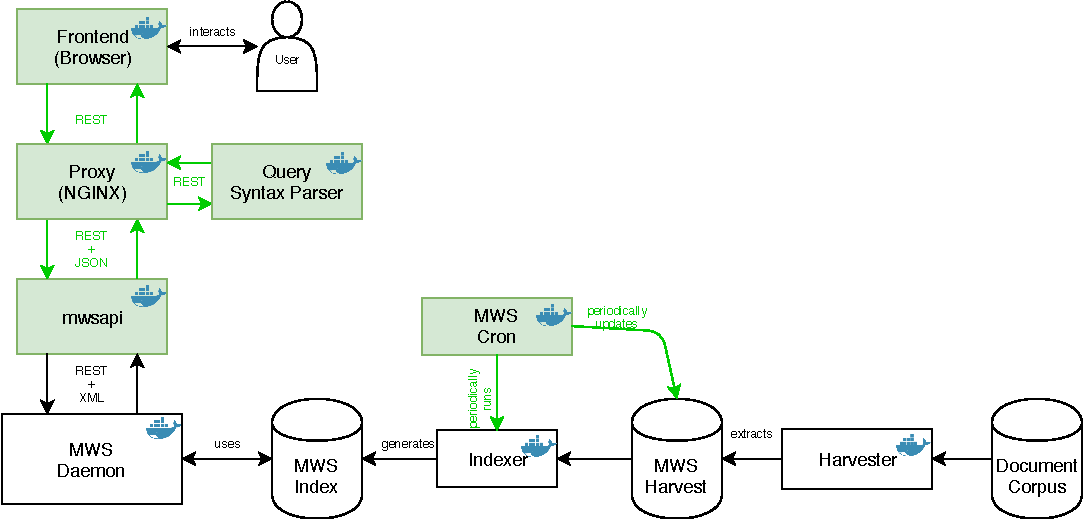
\includegraphics[width=0.8\textwidth]{mws_layout.pdf}
  \caption{Structure of a typical MathWebSearch Deployment}\label{fig:mwsdeployment}
\end{figure}

We describe the components of our infrastructure. 

\paragraph{The MathWebSearch Daemon}
The central component is the \textit{MathWebSearch daemon}, which can be found in the bottom left. 
As previously, it uses an \textit{Index} and exposes an XML-based API for queries. 
The only change we made to the core daemon is that it now exists inside a Docker Container. 

\paragraph{The Harvesters and The Indexer}
In order to generate an index from a set of documents, as before, we need two components. 
First we extract a set of ContentMathML formulae using a corpus-specific \textit{Harvester} (bottom right). 
The generated \textit{Harvest} is then sent to the \textit{Indexer} (bottom center), which generates or updates the \textit{Index}. 

Additionally, we introduced a scheduler component called \textit{MWS cron}. 
This periodically sends updated harvests to the \textit{indexer}, which then in turn updates the index. 
This process ensures that the Index remains up-to-date. 

\paragraph{Frontend, mwsapi and the query syntax parser}

In order to process end user queries, we introduced several additional components.

The most important component of these is the \textit{frontend}, which runs inside the users' browser. 
It allows users to enter a formula search query, and view the results. 
The frontend contains corpus-specific branding and text, and is otherwise not corpus-specific. 
In particular the querying code which interacts with the backend components, does not require specialization. 
\ednote{Screenshot here?}

While the MathWebSearch daemon only understands formulae in Content MathML, users often enter them using different representations, such as \LaTeX. 
For this purpose, the frontend allows entering queries in human-writable, corpus-specific syntax. 
In order to transform the user query into a system-understood query, we make use of a new component called the \textit{Query Syntax Parser}. 
For {\LaTeX} syntax this is achieved using {\LaTeX}ML along with a custom MathWebSearch extension, but this component is fully interchangable if the user desires other syntaxes. 

The frontend does not directly send MathML queries to the \textit{Daemon}.
Instead, it sends them to a thin API layer on top called \textit{mwsapi}. 
This layer forwards the queries to the daemon and, upon receiving a response, performs some post-processing. 
This process includes transforming substiutions returned by MathWebSearch into a format that can be directly presented to the user by the frontend. 

As the frontend, the mwsapi server and the Query Syntax Presenter are all exposed to the end-user under the same url, a proxy delegating requests accordingly was also neccessary. 
This is using an nginx \ednote{cite} server. 

\subsection{Building a Notebook Search}

For certain situations Sage can produce \LaTeX formulae as output. 
To enable search on these formulae, we developed a harvester and used it in our MathWebSearch infrastructure. 

The harvester takes as input a single Sage Jupyter Notebook, and produces a MathWebSearch Harvest of ContentMathML formulae. 
It achieves this by processing each individual LaTeX formula using LaTeXML. 
We then connected this harvester to the GitHub API and used it to harvest formulae from \ednote{conceptually all, but this part isn't fully fleshed out, hence at the moment only a subset} Sage Jupyter Notebooks on GitHub. 

\ednote{
yet to do:
- deployed this using customized branding
- screenshot + url
- evalutation: this was easy to do and gave a large benefit to the community
}

\subsection{Future Plans for MathWebSearch}

- describe the custom component / frontends for NLAB
- temasearch
- python ast search + input syntax?

%%% Local Variables:
%%% mode: latex
%%% mode: visual-line
%%% fill-column: 5000
%%% TeX-master: "report"
%%% End:
